\begin{flushright} {\tiny {\color{gray} nlconvcrit.tex}} \end{flushright}

Disclaimer: the topic of nonlinear PDEs solving is vast and has received 
much attention from the mathematical community. In what follows I present 
a few key ideas which are at the core of many codes and publications in 
computational geodynamics.

Looking at the conservation equations that we must solve, i.e. 
conservation of mass, momentum and energy, we find that more often 
than not the coefficients of these PDEs depend on the strain rate, 
temperature, pressure, etc ... 
This makes solving the PDEs even harder. 
Also the advection term $\vec{\upnu}\cdot \vec\nabla$ couples the two primary 
variables velocity and temperature. 

One simple approach consists first in 'separating' the mass+momentum equations 
from the energy equation: one solves the first two equations assuming temperature known
while the energy equation is solved assuming velocity and pressure known. 
Better schemes obviously exist and iterate on these equations until convergence 
for velocity, pressure and temperature is reached (see for instance the \aspect manual). 
In what follows I focus on the mass and momentum equations assuming temperature known. 

The main source of nonlinearity lies in the (effective) viscosity which often
depends on strain rate and pressure (note that density can also depend on pressure
in compressible cases):
\begin{eqnarray}
\vec\nabla\cdot (2 \eta_{\rm eff}(\dot{\bm\varepsilon},p) \;  \dot{\bm\varepsilon}) 
- \vec\nabla p + \rho \vec{g} &=& \vec{0} \nn\\
\vec\nabla \cdot \vec\upnu &=& 0\nn
\end{eqnarray}
Simply put, in order to solve these equations and obtain 
the velocity and pressure fields I need to specify the density and viscosity (and of course 
appropriate boundary conditions!), but in order to compute the viscosity I need the strain rate 
and pressure fields.  

The simplest approach here consists in so-called Picard iterations as 
explained in Section~\ref{ss:picard}.

Let us start with the penalty-based FEM codes. In this case the mass and momentum 
equations are 'merged' into a single PDE where pressure has been eliminated:
\[
\vec\nabla\cdot (2 \eta_{\rm eff}(\dot{\bm\varepsilon},p) \;  \dot{\bm\varepsilon}) 
+\lambda \vec\nabla (\vec\nabla \cdot \vec\upnu) + \rho \vec{g} = \vec{0} 
\]
In this case the algorithm is simple:
\begin{enumerate}
\item start with a guess for the velocity and pressure fields, i.e. $\vec{\cal V}^{old}$ 
and $\vec{\cal P}^{old}$
\item compute the effective viscosity field with $\vec{\cal V}^{old}$ and $\vec{\cal P}^{old}$
\item solve PDE, obtain new solution $\vec{\cal V}^{new}$ 
\item compute $\vec{\cal P}^{new}$ from $\vec{\cal V}^{new}$
\item assess convergence, i.e. answer 'how close are the newly obtained fields from the old ones?'
\item $\vec{\cal V}^{old} \leftarrow \vec{\cal V}^{new}$, and $\vec{\cal P}^{old} \leftarrow \vec{\cal P}^{new}$
\item if not converged go back to 2, else exit
\end{enumerate}

Thieulot (2011) \cite{thie11} computes the means
$\langle \vec{\cal V}^i\rangle$, 
$\langle \vec{\cal V}^{i+1}\rangle$, 
and the variances 
$\sigma_{\cal V}^i$ and 
$\sigma_{\cal V}^{i+1}$ 
followed by the correlation 
\[
R^{i,i+1} = \frac{\langle (\vec{\cal V}^i - \langle \vec{\cal V}^i\rangle)
\cdot ( \vec{\cal V}^{i+1} - \langle \vec{\cal V}^{i+1}\rangle) \rangle }
{\sqrt{\sigma_{\cal V}^i \sigma_{\cal V}^{i+1}}}
\]
Since the correlation is normalised, it takes values between 0
(very dissimilar velocity fields) and 1 (very similar fields). The
following convergence criterion, formulated in terms of the variable $\chi = 1 -R^{i,i+1} $
has been implemented: convergence is reached when $\chi>tol$.
Since pressure is a derived quantity from velocity, if velocity is converged so is 
pressure\footnote{Two caveats here: the amplitude of the chequerboard mode
might come into play - in the case $Q_1\times P_0$ elements are used- and so does the applied smoothing.}.

When the algorithm above is close to convergence then $\vec{\cal V}^i$ and $\vec{\cal V}^{i-1}$ are close. 
If these were scalar quantities we could subtract them and look at the (absolute) difference: 
if it is 'small enough' then the algorithm has converged. 
However there are two problems with this: 
\begin{enumerate}
\item $\vec{\cal V}^i$ and $\vec{\cal V}^{i-1}$ are vector 
quantities (with potentially millions of values) so in order to measure a scalar difference 
between these we must take the norm of the difference, or $||\vec{\cal V}^i-\vec{\cal V}^{i-1}||$
and it is common to take the $L^2$-norm. 
\item we do not know a priori the (magnitude of the) solution so that 'small enough' is a dangerous 
statement. We could check for $||\vec{\cal V}^i-\vec{\cal V}^{i-1}||<tol$ and set $tol=10^{-6}$
for example. However in geodynamics velocities are of the order of a \si{\cm\per\year} which is 
about $3.1\cdot10^{-10}\si{\metre\per\second}$. Small velocity changes would then be enforced
only if $tol<10^{-12}$. This value might prove completely unpractical for other applications. 
In light of all this one then resorts to assessing the {\it relative} change in the velocity by normalising 
the previous quantity by the average velocity in the domain $||\vec{\cal V}^i||$.
\end{enumerate}

This is the very approach taken by Spiegelman \etal \cite{spmw16} who monitor the 
relative changes in the solution from iteration to iteration: 
\[
\frac{||\Delta \vec{\cal V} ||_{L2}}{||\vec{\cal V}||_{L2}} 
=
\left( \frac{\int\limits_\Omega (\vec{\cal V}_i-\vec{\cal V}_{i-1}) \cdot( \vec{\cal V}_i-\vec{\cal V}_{i-1}) dV}{\int\limits_\Omega \vec{\cal V}_i\cdot\vec{\cal V}_i dV} \right)^{1/2}
\]
Of course, if a mixed formulation is used where velocity and pressure are solved for unknowns,
the same monitoring can be done for pressure:
\[
\frac{||\Delta \vec{\cal P} ||_{L2}}{||\vec{\cal P}||_{L2}} 
=
\left( \frac{\int\limits_\Omega (\vec{\cal P}_i-\vec{\cal P}_{i-1}) \cdot( \vec{\cal P}_i-\vec{\cal P}_{i-1}) dV}{\int\limits_\Omega \vec{\cal P}_i\cdot\vec{\cal P}_i dV} \right)^{1/2}
\]
Convergence is reached when both are below 0.001 (as in Lemiale \etal (2008) \cite{lemm08}) 
or 0.0001 (as in Kaus \etal (2010) \cite{kaus10}).

The last option is via the nonlinear residual. Coming back to the penalty formulation, 
we can form the nonlinear residual as follows:
\[
\vec{\cal R}^i = \K(\eta_{\rm eff}(\dot{\bm\varepsilon}^{i-1},p^{i-1})) \cdot \vec{\cal V}^i - \vec{f}
\]
where $\K$ is defined in Section~\ref{sec_penalty}. 
Close to convergence $\vec{\cal V}^i$ and $\vec{\cal V}^{i-1}$
are very close so that we expect the residual $\vec{\cal R}$ to become smaller and smaller.
In order to extract a scalar from $\vec{\cal R}$ we once again resort to the $L^2$-norm and 
we also wish to to monitor its relative change. In this case it is customary to use $\vec{\cal R}^0$ so 
that the convergence criterion becomes
\[
\frac{||\vec{\cal R}^i ||}{||\vec{\cal R}^0 ||} < tol.
\]

FINISH: explain problem with mixed formulation!


\begin{center}
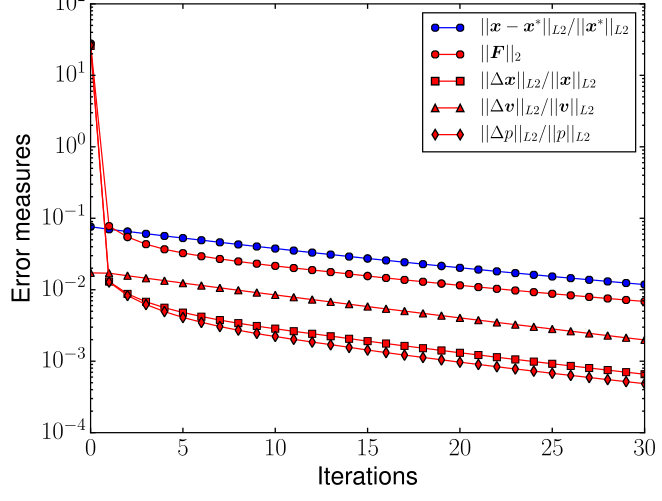
\includegraphics[width=6cm]{images/nlconv/spmw16}\\
{\captionfont Taken from Spiegelman, May \& Wilson \etal (2016). Example of 
reported nonlinear convergence.}
\end{center}





